%%%%%%%%%%%%%%%%%%%%%%%%%%%%%%%%%%%%%%%%%
% Beamer Presentation
% LaTeX Template
% Version 2.0 (March 8, 2022)
%
% This template originates from:
% https://www.LaTeXTemplates.com
%
% Author:
% Vel (vel@latextemplates.com)
%
% License:
% CC BY-NC-SA 4.0 (https://creativecommons.org/licenses/by-nc-sa/4.0/)
%
%%%%%%%%%%%%%%%%%%%%%%%%%%%%%%%%%%%%%%%%%

%----------------------------------------------------------------------------------------
%	PACKAGES AND OTHER DOCUMENT CONFIGURATIONS
%----------------------------------------------------------------------------------------

\documentclass[
	11pt, % Set the default font size, options include: 8pt, 9pt, 10pt, 11pt, 12pt, 14pt, 17pt, 20pt
	%t, % Uncomment to vertically align all slide content to the top of the slide, rather than the default centered
	%aspectratio=169, % Uncomment to set the aspect ratio to a 16:9 ratio which matches the aspect ratio of 1080p and 4K screens and projectors
]{beamer}

% Hide navigation symbols
\setbeamertemplate{navigation symbols}{}

\usepackage{caption}
\captionsetup[figure]{labelsep=space}
\renewcommand{\figurename}{}
\renewcommand{\tablename}{}
\graphicspath{{images/}{./}} % Specifies where to look for included images (trailing slash required)
% \usepackage{minted}
\usepackage{booktabs} % Allows the use of \toprule, \midrule and \bottomrule for better rules in tables

%----------------------------------------------------------------------------------------
%	SELECT LAYOUT THEME
%----------------------------------------------------------------------------------------

% Beamer comes with a number of default layout themes which change the colors and layouts of slides. Below is a list of all themes available, uncomment each in turn to see what they look like.

%\usetheme{default}
%\usetheme{AnnArbor}
%\usetheme{Antibes}
%\usetheme{Bergen}
%\usetheme{Berkeley}
% \usetheme{Berlin}
%\usetheme{Boadilla}
% \usetheme{CambridgeUS}
% \usetheme{Copenhagen}
% \usetheme{Darmstadt}
% \usetheme{Dresden}
% \usetheme{Frankfurt}
% \usetheme{Goettingen}
% \usetheme{Hannover}
% \usetheme{Ilmenau}
% \usetheme{JuanLesPins}
% \usetheme{Luebeck}
\usetheme{Madrid}
%\usetheme{Malmoe}
%\usetheme{Marburg}
%\usetheme{Montpellier}
%\usetheme{PaloAlto}
%\usetheme{Pittsburgh}
%\usetheme{Rochester}
%\usetheme{Singapore}
%\usetheme{Szeged}
%\usetheme{Warsaw}

%----------------------------------------------------------------------------------------
%	SELECT COLOR THEME
%----------------------------------------------------------------------------------------

% Beamer comes with a number of color themes that can be applied to any layout theme to change its colors. Uncomment each of these in turn to see how they change the colors of your selected layout theme.

% \usecolortheme{albatross}
% \usecolortheme{beaver}
% \usecolortheme{beetle}
% \usecolortheme{crane}
% \usecolortheme{dolphin}
% \usecolortheme{dove}
% \usecolortheme{fly}
% \usecolortheme{lily}
% \usecolortheme{monarca}
% \usecolortheme{seagull}
% \usecolortheme{seahorse}
\usecolortheme{spruce}
% \usecolortheme{whale}
% \usecolortheme{wolverine}

%----------------------------------------------------------------------------------------
%	SELECT FONT THEME & FONTS
%----------------------------------------------------------------------------------------

% Beamer comes with several font themes to easily change the fonts used in various parts of the presentation. Review the comments beside each one to decide if you would like to use it. Note that additional options can be specified for several of these font themes, consult the beamer documentation for more information.

\usefonttheme{default} % Typeset using the default sans serif font
%\usefonttheme{serif} % Typeset using the default serif font (make sure a sans font isn't being set as the default font if you use this option!)
\usefonttheme{structurebold} % Typeset important structure text (titles, headlines, footlines, sidebar, etc) in bold
%\usefonttheme{structureitalicserif} % Typeset important structure text (titles, headlines, footlines, sidebar, etc) in italic serif
%\usefonttheme{structuresmallcapsserif} % Typeset important structure text (titles, headlines, footlines, sidebar, etc) in small caps serif

%------------------------------------------------

%\usepackage{mathptmx} % Use the Times font for serif text
\usepackage{palatino} % Use the Palatino font for serif text

%\usepackage{helvet} % Use the Helvetica font for sans serif text
\usepackage[default]{opensans} % Use the Open Sans font for sans serif text
%\usepackage[default]{FiraSans} % Use the Fira Sans font for sans serif text
%\usepackage[default]{lato} % Use the Lato font for sans serif text

%----------------------------------------------------------------------------------------
%	SELECT INNER THEME
%----------------------------------------------------------------------------------------

% Inner themes change the styling of internal slide elements, for example: bullet points, blocks, bibliography entries, title pages, theorems, etc. Uncomment each theme in turn to see what changes it makes to your presentation.

%\useinnertheme{default}
\useinnertheme{circles}
% \useinnertheme{rectangles}
% \useinnertheme{rounded}
%\useinnertheme{inmargin}

%----------------------------------------------------------------------------------------
%	SELECT OUTER THEME
%----------------------------------------------------------------------------------------

% Outer themes change the overall layout of slides, such as: header and footer lines, sidebars and slide titles. Uncomment each theme in turn to see what changes it makes to your presentation.

% \useoutertheme{default}
% \useoutertheme{infolines}
\useoutertheme{miniframes}
% \useoutertheme{smoothbars}
% \useoutertheme{sidebar}
%\useoutertheme{split}
% \useoutertheme{shadow}
% \useoutertheme{tree}
%\useoutertheme{smoothtree}

%\setbeamertemplate{footline} % Uncomment this line to remove the footer line in all slides
%\setbeamertemplate{footline}[page number] % Uncomment this line to replace the footer line in all slides with a simple slide count

%\setbeamertemplate{navigation symbols}{} % Uncomment this line to remove the navigation symbols from the bottom of all slides

%----------------------------------------------------------------------------------------
%	PRESENTATION INFORMATION
%----------------------------------------------------------------------------------------

\title[LAB 01: Introduction to MARS]{LAB 01: Introduction to MARS} % The short title in the optional parameter appears at the bottom of every slide, the full title in the main parameter is only on the title page

% \subtitle{Optional Subtitle} % Presentation subtitle, remove this command if a subtitle isn't required

\author[S. AlSaleh]{Saleh AlSaleh \\ \smallskip \textit{salehs@kfupm.edu.sa}} % Presenter name(s), the optional parameter can contain a shortened version to appear on the bottom of every slide, while the main parameter will appear on the title slide

\institute[KFUPM]{King Fahd University of Petroleum and Minerals \\ College of Computing and Mathematics \\ Computer Engineering Department} % Your institution, the optional parameter can be used for the institution shorthand and will appear on the bottom of every slide after author names, while the required parameter is used on the title slide and can include your email address or additional information on separate lines

\date[January 15, 2023]{COE301: Computer Architecture \\ Term 222} % Presentation date or conference/meeting name, the optional parameter can contain a shortened version to appear on the bottom of every slide, while the required parameter value is output to the title slide

%----------------------------------------------------------------------------------------

\begin{document}

%----------------------------------------------------------------------------------------
%	TITLE SLIDE
%----------------------------------------------------------------------------------------

\begin{frame}
	% Output the title slide, automatically created using the text entered in the PRESENTATION INFORMATION block above
	\titlepage
\end{frame}

%----------------------------------------------------------------------------------------
%	TABLE OF CONTENTS SLIDE
%----------------------------------------------------------------------------------------

% The table of contents outputs the sections and subsections that appear in your presentation, specified with the standard \section and \subsection commands. You may either display all sections and subsections on one slide with \tableofcontents, or display each section at a time on subsequent slides with \tableofcontents[pausesections]. The latter is useful if you want to step through each section and mention what you will discuss.

\begin{frame}
	\frametitle{Agenda} % Slide title, remove this command for no title
	
	\tableofcontents % Output the table of contents (all sections on one slide)
	%\tableofcontents[pausesections] % Output the table of contents (break sections up across separate slides)
\end{frame}

%----------------------------------------------------------------------------------------
%	PRESENTATION BODY SLIDES
%----------------------------------------------------------------------------------------

\section{Personal Information} % Sections are added in order to organize your presentation into discrete blocks, all sections and subsections are automatically output to the table of contents as an overview of the talk but NOT output in the presentation as separate slides

%------------------------------------------------

% \subsection{Paragraphs and Lists}

\begin{frame}
	\frametitle{Personal Information}
	
	\begin{itemize}
		\item Name            : Saleh AlSaleh
		\item Office Phone    : +966-13-860-7035
		\item Office Location : Building 23 Room 10-4
		\item Office Hours    : Tuesday and Wednesday 12:30-01:30 PM or by appointment. 
	\end{itemize}

\end{frame}

%------------------------------------------------

\section{Introduction}
\begin{frame}
	\frametitle{Introduction}
	\begin{columns}[c] % The "c" option specifies centered vertical alignment while the "t" option is used for top vertical alignment
		\begin{column}{0.65\textwidth} % Left column width
			\begin{itemize}
				\item In this lab we will learn about 32-bit MIPS RISC (Reduced Instruction Set Computer) CPU.
				\item Popular Systems with MIPS CPU: Nintendo 64, Sony Playstation (Origianl), Sony PlayStation 2, and Sony PlayStation Portable (PSP).
				\item Common Uses for MIPS CPU: Embedded Systems, routers, and switches.
			\end{itemize}
		\end{column}
		
		\begin{column}{0.35\textwidth} % right column width
			\begin{figure}
				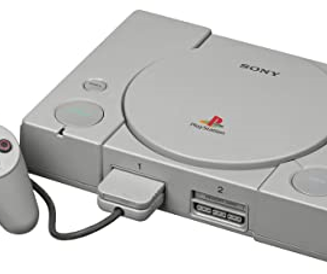
\includegraphics[width=0.5\linewidth]{ps1.png}
				\caption{Sony Playstation 1}
			\end{figure}
			\begin{figure}
				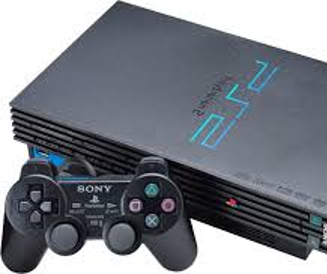
\includegraphics[width=0.5\linewidth]{ps2.png}
				\caption{Sony Playstation 2}
			\end{figure}
		\end{column}
	\end{columns}
\end{frame}

\begin{frame}
	\frametitle{Introduction}
	\begin{columns}[c] % The "c" option specifies centered vertical alignment while the "t" option is used for top vertical alignment
		\begin{column}{0.6\textwidth} % Left column width
			\begin{itemize}
				\item Assembly Language is the lowest level of programming for CPUs. 
				\item In most cases, each assembly instruction maps to one specific operation.
				\item An Assembler is needed to convert the assembly code to binary (0 and 1).
				\item MIPS has 32 General Purpose Registers: \$ 0 to \$ 31.
				\item Some of these registers have specific functionality (e.g. \$ sp stack pointer).
			\end{itemize}
		\end{column}
	
		\begin{column}{0.4\textwidth} % right column width
			% \begin{exampleblock}{MIPS Sample Code}
			% 	\begin{minted}
			% 		loop: 	lw   $t3, 0($t0)
			% 				lw   $t4, 4($t0)
			% 				add  $t2, $t3, $t4
			% 				sw   $t2, 8($t0)
			% 				addi $t0, $t0, 4
			% 				addi $t1, $t1, -1
			% 				bgtz $t1, loop
			% 	\end{minted}
			% \end{exampleblock}
			\begin{figure}
				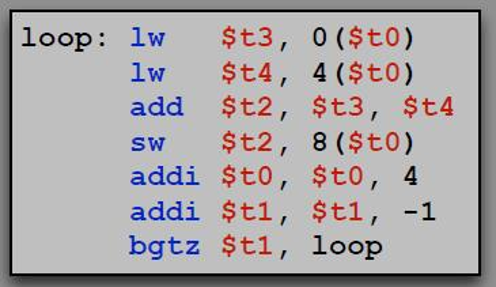
\includegraphics[width=\linewidth]{mips_sample_code.png}
				\caption{MIPS Sample Code}
			\end{figure}
		\end{column}
	\end{columns}
\end{frame}

%------------------------------------------------

\section{MARS Simulator}
\begin{frame}
	\frametitle{MARS Simulator}
	
	\begin{itemize}
		\item MARS is a MIPS Assembly and Runtime Simulator.
		\item MARS is an integrated development environment (IDE) for programming in MIPS assembly language.
		\item MARS allows editing, assembling, debugging and simulating the execution of MIPS assembly language programs.
		\item MARS is written in Java, so it can be run on Windows, macOS, and Linux.
		\item There are two main windows in MARS: \textbf{Edit} Window and \textbf{Execute} Window.
	\end{itemize}
\end{frame}

%------------------------------------------------

\section{Demo}

\begin{frame}
	\frametitle{Demo}
	
\end{frame}

%------------------------------------------------

\section{Grade Distribution}

\begin{frame}
	\frametitle{Grade Distribution}
	\begin{table}
		\begin{tabular}{l c}
			\toprule
			\textbf{Activity} & \textbf{Weight} \\
			\midrule
			Lab Tasks (8 Experiments)     	& 12 \\
			Lab Quizzes (Best 3 out of 4) 	& 3 \\
			\bottomrule
			Total 							& 15 \\
		\end{tabular}
		\caption{Lab Work Grade Distribution}
	\end{table}
	\begin{table}
		\begin{tabular}{l c}
			\toprule
			\textbf{Activity} & \textbf{Weight} \\
			\midrule
			Single Cycle CPU Design              &  8 \\
			Pipelined CPU Design                 &  5 \\
			Report                               &  2 \\
			\bottomrule
			Total 					             & 15 \\
		\end{tabular}
		\caption{Lab Project Grade Distribution}
	\end{table}
\end{frame}

%----------------------------------------------------------------------------------------

\end{document} 